This chapter discusses proposed transition scenarios for new nuclear reactor deployment in the \gls{usa} and the reactor models used to simulate them. It also discusses the theoretical framework and key concepts that underpin the research and the results for each deployment scheme.

\section{Transition Scenarios}
\label{sec:transition_scenarios}
% Discuss the theoretical framework and key concepts that underpin the research.

This chapter explores the deployment schemes implemented in this thesis---outlined in Table \ref{tab:deployment_schemes}---and the demand growth scenarios that this thesis considered---outlined in Table \ref{tab:demand_scenarios}. Appendix \ref{sec:considered_deployment_schemes} will discuss two additional deployment schemes that I implemented but did not leverage, as they are more useful for problems not considered herein.

As the energy landscape evolves, compounding factors will drive the actual deployment of these reactors in ways this thesis does not capture. The value of energy system modeling and transition scenarios is to understand the deployment implications compared with and measured relative to business-as-usual cases with similar approximations.

\begin{table}[H]
    \centering
    \caption{Deployment schemes.}
    \label{tab:deployment_schemes}
    \begin{tabular}{p{0.15\linewidth} >{\raggedright}p{0.20\linewidth}>{\raggedright\arraybackslash}p{0.50\linewidth}}
        \hline
        Status & Scheme & Description \\
        \hline
        & Greedy Deployment & Deploy reactors to fill demand, preferring to deploy larger capacity units first. \\
        Incorporated & Random Deployment & Uses a date and hour as seed to sample the
        reactors list randomly. \\
        & Initially Random then Greedy Deployment & Randomly deploy reactors until
        a reactor bigger than the remaining capacity is proposed for each time step,
        then fills the remaining capacity with the greedy algorithm. \\
        % & Single Reactor & A single reactor model is deployed as the existing fleet is decommissioned.\\
        \hline
         & Capped Deployment & There is a
        single-number capacity for one or more of the reactor models. \\
        Not Incorporated & Pre-Determined Distribution Deployment & One or more reactors have a
        preset distribution, and a smaller capacity model fills in the gaps. \\
        \hline
    \end{tabular}
\end{table}

These deployment schemes choose reactors to fill demand growth based on two predictions of future. The \gls{eia} publishes demand expansion projections for the totality of the \gls{usa} \cite{eia_aeo_2023}. The administration has refrained from publishing AEO 2024 in light of recent accelerations in demand growth. The assumptions for the low-growth scenarios are that the relative percentage of nuclear power remains constant and that the relative performance of the various fuel cycle metrics will remain constant. The high-growth scenarios come from the \gls{doe} Liftoff Report \cite{julie_liftoff_pathways_2024}, which does not reflect this constant percentage assumption for nuclear power in their demand scenarios. Their growth projections are specific to nuclear energy deployment increases, and the number is agnostic to the total increase.

\begin{table}[H]
    \centering
    \caption{Demand growth scenarios.}
    \label{tab:demand_scenarios}
    \begin{tabular}{l l l}
        \hline
        \textbf{Demand Growth} & \textbf{Year-to-Year Increase} & \textbf{Source}\\
        \hline
        No Growth & 0.0\% & N/A\\
        Low Growth & 0.17\% & \cite{eia_aeo_2023}\\
        Low Growth & 0.5\% & \cite{eia_aeo_2023}\\
        Low Growth & 1.0\% & \cite{eia_aeo_2023}\\
        High Growth & 3.5\% & \cite{julie_liftoff_pathways_2024} \\
        High Growth & 5.6\% & \cite{julie_liftoff_pathways_2024}\\
        \hline
    \end{tabular}
  \end{table}

As shown in Table \ref{tab:simulations}, each growth scenario has two enrichment deployments: 1) the reactors are never fueled with \gls{leup}; 2) the \gls{mmr} and \gls{xe} reactors are fueled with \gls{leup} until 2040, when they move to \gls{haleu}. \glspl{mmr} deployed before this fuel transition will continue to use \gls{leup} fuel until the end of their lifetime as they do not refuel; however, the \gls{xe} reactors will refuel with \gls{leup} until 2040, when they will refuel with \gls{haleu}. The AP1000 reactors will continue to use \gls{leu} fuel throughout the simulation.

\begin{longtable}[c]{l l l l}
    \caption{Transition scenario simulations run.} \label{tab:simulations} \\
    \hline
    \textbf{Run} & \textbf{Deployment Scheme} & \textbf{Demand Growth} & \textbf{Fuel Choice} \\
    \hline
    \endfirsthead

    \hline
    \textbf{Run} & \textbf{Deployment Scheme} & \textbf{Demand Growth} & \textbf{Fuel Choice} \\
    \hline
    \endhead

    \hline
    \endfoot

    \hline
    \endlastfoot
    \RomanNumeralCaps{1} & Greedy & 0.0\% & Single\\
        \RomanNumeralCaps{2} & Greedy & 0.0\% & Multi\\
        \RomanNumeralCaps{3} & Greedy & 0.17\% & Single\\
        \RomanNumeralCaps{4} & Greedy & 0.17\% & Multi\\
        \RomanNumeralCaps{5} & Greedy & 0.5\% & Single\\
        \RomanNumeralCaps{6} & Greedy & 0.5\% & Multi\\
        \RomanNumeralCaps{7} & Greedy & 1.0\% & Single\\
        \RomanNumeralCaps{8} & Greedy & 1.0\% & Multi\\
        \RomanNumeralCaps{9} & Greedy & 3.5\% & Single\\
        \RomanNumeralCaps{10} & Greedy & 3.5\% & Multi\\
        \RomanNumeralCaps{11} & Greedy & 5.6\% & Single\\
        \RomanNumeralCaps{12} & Greedy & 5.6\% & Multi\\
        \hline
        \RomanNumeralCaps{13} & Random & 0.0\% & Single\\
        \RomanNumeralCaps{14} & Random & 0.0\% & Multi\\
        \RomanNumeralCaps{15} & Random & 0.17\% & Single\\
        \RomanNumeralCaps{16} & Random & 0.17\% & Multi\\
        \RomanNumeralCaps{17} & Random & 0.5\% & Single\\
        \RomanNumeralCaps{18} & Random & 0.5\% & Multi\\
        \RomanNumeralCaps{19} & Random & 1.0\% & Single\\
        \RomanNumeralCaps{20} & Random & 1.0\% & Multi\\
        \RomanNumeralCaps{21} & Random & 3.5\% & Single\\
        \RomanNumeralCaps{22} & Random & 3.5\% & Multi\\
        \RomanNumeralCaps{23} & Random & 5.6\% & Single\\
        \RomanNumeralCaps{24} & Random & 5.6\% & Multi\\
        \hline
        \RomanNumeralCaps{25} & Random + Greedy & 0.0\% & Single\\
        \RomanNumeralCaps{26} & Random + Greedy & 0.0\% & Multi\\
        \RomanNumeralCaps{27} & Random + Greedy & 0.17\% & Single\\
        \RomanNumeralCaps{28} & Random + Greedy & 0.17\% & Multi\\
        \RomanNumeralCaps{29} & Random + Greedy & 0.5\% & Single\\
        \RomanNumeralCaps{30} & Random + Greedy & 0.5\% & Multi\\
        \RomanNumeralCaps{31} & Random + Greedy & 1.0\% & Single\\
        \RomanNumeralCaps{32} & Random + Greedy & 1.0\% & Multi\\
        \RomanNumeralCaps{33} & Random + Greedy & 3.5\% & Single\\
        \RomanNumeralCaps{34} & Random + Greedy & 3.5\% & Multi\\
        \RomanNumeralCaps{35} & Random + Greedy & 5.6\% & Single\\
        \RomanNumeralCaps{36} & Random + Greedy & 5.6\% & Multi\\
        \hline
    \end{longtable}

Under each enrichment deployment, each demand projection is met by deploying reactors using the
schemes outlined in Table \ref{tab:deployment_schemes}. The following sections will discuss the results of these deployment schemes, their limitations, and propose future work. Regardless of the enrichment deployment, each run will attempt to deploy reactors to meet the capacity outlined in Figure \ref{fig:dep_goals}. The results will focus on the \textit{no growth} and $3.5\%$ growth (corresponding to doubling nuclear by 2050) scenarios.

\begin{figure}[H]
    \centering
    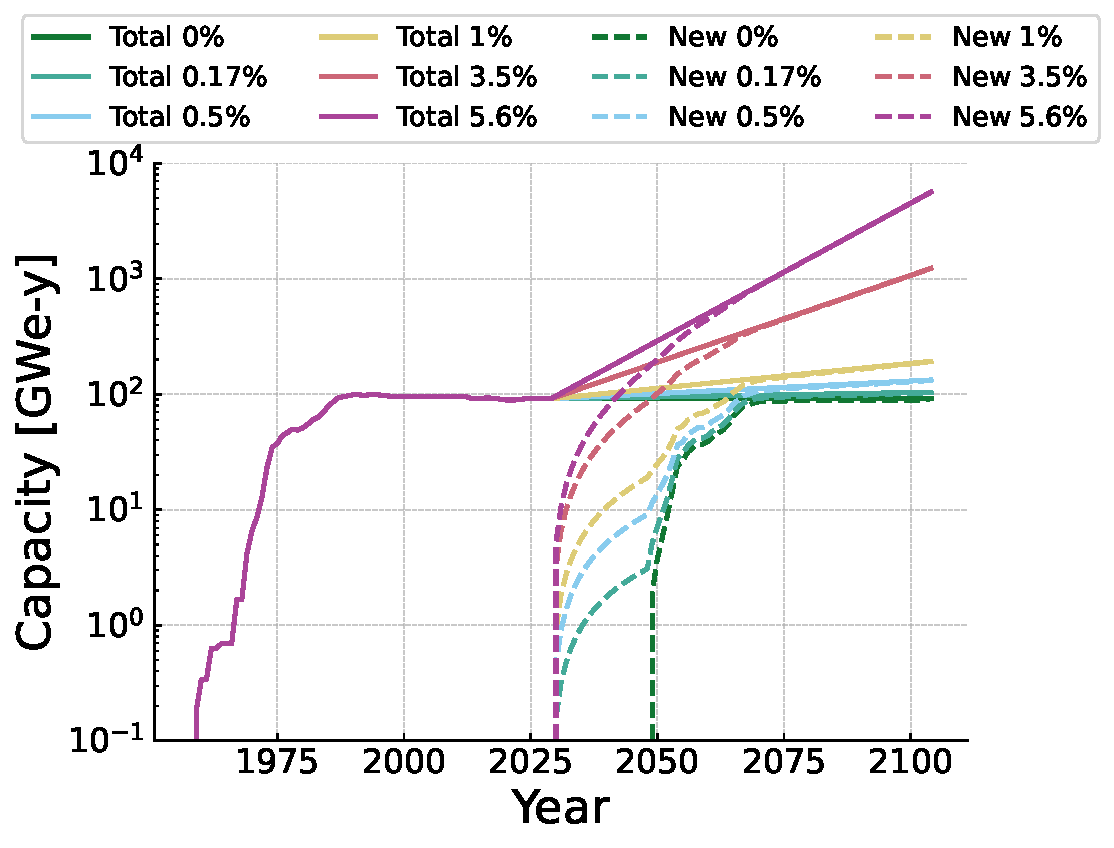
\includegraphics[scale=0.7]{images/results/deployment_calcs/total_new_capacity_scenarios.pdf}
    \caption{Total and new nuclear capacity deployed in each scenario.}
    \label{fig:dep_goals}
\end{figure}

As shown, advanced reactors (for this thesis, the designs are the \gls{mmr},
\gls{xe}, and AP1000) begin deployment in 2030. While this is an aggressive deployment schedule, \cite{bachmann_thesis_2023} established that the precise deployment start did not significantly impact the total results for this type of analysis and could reasonably serve as an upper bound of deployment. The business-as-usual, or \textit{no growth}, scenario does not require the deployment of a new nuclear reactor until just before 2050, whereas the other scenarios understandably commence deployment in 2030. As it is on a logarithmic plot, the linear appearance of the data belies the compounding effect that the year-to-year percentage growth requires.

Comparing these projected deployments with the results from the \textit{no growth} and \textit{double by 2050} scenarios, Table \ref{tab:cap_diff} consolidates the over- and under- deployments of capacity into Table to show that the random deployment scheme had the least total difference between the results and the projection. The initially random, then greedy deployment scheme showed the largest total difference between the results and the projection, while the greedy deployment scheme was between the two.

\begin{table}[H]
    \centering
    \caption{Capacity difference between results and projection.}
    \label{tab:cap_diff}
    \begin{tabular}{l l l}
        \hline
        % \multicolumn{1}{c}{\textbf{Scenario} & \textbf{Deployment Scheme} & \textbf{Total Difference [GWe]}}\\
        \textbf{Scenario} & \textbf{Deployment Scheme} & \textbf{Total Difference [GWe]}\\
        \hline
        \multirow{3}{*}{No Growth} & Greedy & \textcolor{white}{0}19.46 \\
        & Random & -15.21 \\
        & Initially Random Then Greedy & \textcolor{white}{0}47.26 \\
        \hline
        \multirow{3}{*}{Double} & Greedy & 103.54 \\
        & Random & \textcolor{white}{00}6.65 \\
        & Initially Random Then Greedy & 151.86 \\
        \hline
    \end{tabular}
\end{table}

Figure \ref{fig:e_diff} shows the difference in energy capacity between the results and the projection for the \textit{no growth} and \textit{double by 2050} scenarios over time. The difference curves in Figure \ref{fig:e_diff_d2} show a tightly perturbed oscillation as more reactors are deployed to meet the increasing demand in the random and the initially random, then greedy schemes. Closer to the start of advanced reactor deployment, the greedy scheme shows a consistently smaller difference than the other schemes, but the difference continues to grow as time progresses.

\begin{figure}[H]
    \subfloat[No Growth. \label{fig:e_diff_ng}]{%
      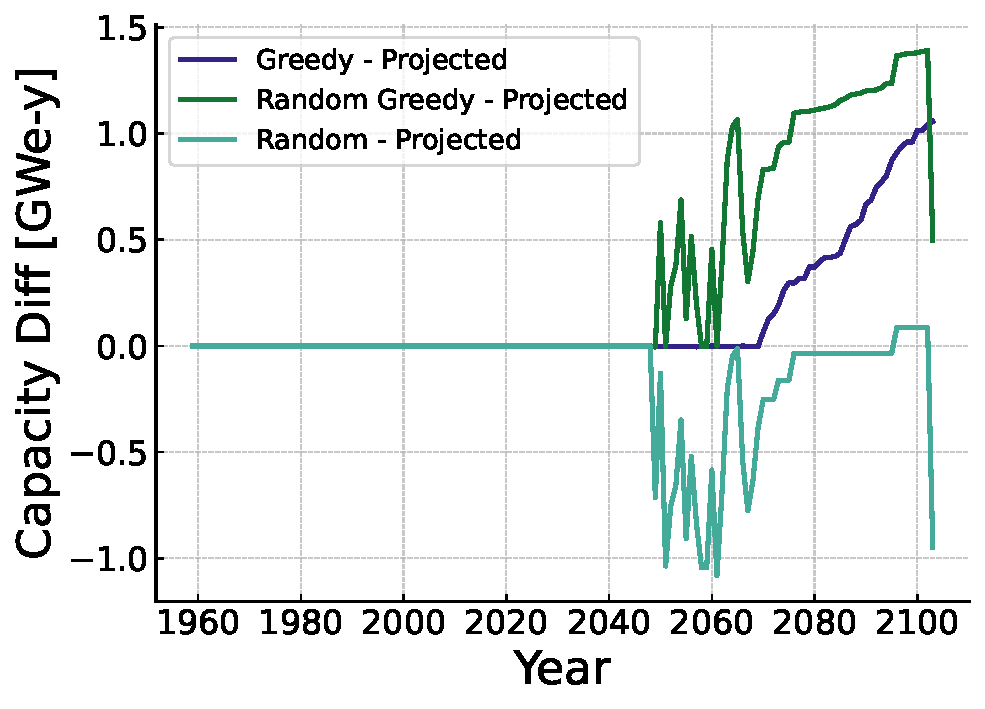
\includegraphics[width=0.495\textwidth]{images/results/energy/ng_diff.pdf}
   }
    \hfill
    \subfloat[Double. \label{fig:e_diff_d2}]{%
      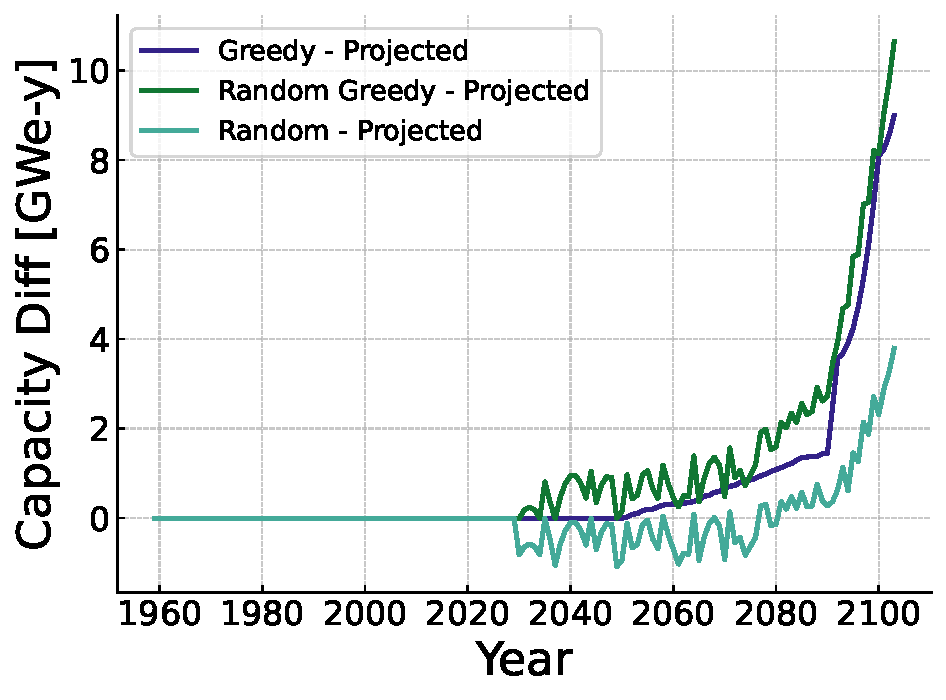
\includegraphics[width=0.495\textwidth]{images/results/energy/d2_diff.pdf}
   }
    \caption{Energy capacity difference between projection and scheme predictions.}
    \label{fig:e_diff}
\end{figure}

